The endeavor to remove specific concepts from diffusion models highlights a critical and multifaceted challenge in the realm of generative artificial intelligence, merging technical sophistication with ethical considerations. As these models increasingly permeate various sectors, the generation of undesired or controversial content raises significant concerns, necessitating interventions that are not only technologically adept but also cognizant of broader societal implications and individual privacy concerns. This complex interplay demands solutions that adeptly navigate the technical intricacies of altering model outputs without compromising on accuracy or creativity, while also ensuring adherence to ethical standards, legal requirements, and cultural sensitivities. As such, the pursuit of concept removal from diffusion models transcends mere algorithmic adjustments, embodying a broader commitment to responsible AI development that respects human values and rights, thereby reinforcing the importance of aligning technological advancements with ethical imperatives in the development and deployment of generative models.

\subsection{Dataset Curation and Post-Hoc Modifications}
Methods to mitigate undesirable image generation have primarily followed two paths. The first approach involves censoring or selectively curating the training dataset to exclude specific classes of images that are considered undesirable, such as removing all images of people or more narrowly targeting specific undesired content \cite{25,39,27,33}. While straightforward, this method is notably resource-intensive due to the significant computational demands of retraining large models. Furthermore, it risks unintended consequences stemming from large-scale censorship \cite{26}.

The alternative, post-hoc strategy modifies the output after training. This can be achieved through the use of classifiers to filter out undesired content \cite{3,21,29} or by incorporating guidance into the inference process \cite{38}. Although these methods are more cost-efficient and quicker to implement, they suffer from vulnerability; knowledgeable users can bypass these safeguards by manipulating model parameters \cite{43}.

In light of these limitations, recent developments have seen the emergence of novel techniques. For example, Stable Diffusion 2.0 represents an effort to retrain models on censored datasets \cite{30}, while Safe Latent Diffusion introduces state-of-the-art guidance-based approaches \cite{38}. Our investigation builds upon these foundations, proposing a third methodology that refines model parameters through a guidance-based model-editing technique, offering both rapid deployment and resilience against circumvention efforts.

\subsection{Image Cloaking}
Image cloaking emerges as a proactive measure enabling content creators to shield their works from being learned by generative models. By introducing adversarial perturbations, artists can obscure their images, effectively disguising them from machine learning algorithms either during training or inference, without impacting human perception significantly \cite{36,42}. This approach, however, diverges from the primary concern of concept removal from the perspective of model creators.

\subsection{Model Editing}
As an extension of concept removal, model editing seeks to adjust the generative capabilities of models without extensive retraining. Techniques vary from modifying specific neurons or layers \cite{7,23} to employing hypernetworks \cite{8,24} for text generators, and analogous methods for image synthesis, such as using textual or sketch inputs, gestures, or direct editing of features \cite{2,14,46,47}. The evolution towards model editing underscores the industry's shift towards more efficient and nuanced control over generative models, aligning with our proposed method of parameter tuning for concept removal.
Among these advancements, the "Forget-Me-Not" \cite*{zhang2023forgetmenot} approach represents a significant stride, utilizing a guidance-based model-editing technique that refines model parameters to selectively forget or correct specific concepts. This method enhances the flexibility and efficiency of concept manipulation in diffusion models, offering a solution that is both quick to deploy and robust against attempts to circumvent concept removal safeguards. The evolution towards model editing, as exemplified by "Forget-Me-Not," underscores the industry's shift towards more efficient and nuanced control over generative models, aligning with our proposed method of parameter tuning for concept removal.



\begin{table}[h]
    \centering
    \label{my-label}
    \begin{tabular}{|l|c|c|c|c|}
    \hline
    \textbf{Methods}      & \textbf{Performance}                     & \textbf{Integrity}                            & \textbf{Generality}                        & \textbf{Flexibility}                 \\ \hline
    Token Blacklisting    & \textcolor{red}{No forgetting}           & \textcolor{yellow}{Inevitably affects}                            & \textcolor{yellow}{Within the}                                 & \textcolor{yellow}{Tokenizer required}                    \\
                          &                                          & \textcolor{yellow}{other concepts}                              & \textcolor{yellow}{vocabulary of the}                        &                                       \\
                          &                                          & \textcolor{yellow}{sharing overlapping}                        & \textcolor{yellow}{tokenizer}                                 &                                       \\
                          &                                          & \textcolor{yellow}{prompts}                                      &                                           &                                       \\ \hline
    Naive Finetuning      & \textcolor{green}{Successfully}          & \textcolor{red}{Removes unrelated}           & \textcolor{green}{Applies to any}          & \textcolor{green}{Applies to any}     \\
                          & \textcolor{green}{removes concept}       & \textcolor{red}{concept by fault}            & \textcolor{green}{concepts with}           & \textcolor{green}{models}             \\
                          &                                          &                                               & \textcolor{green}{sufficient data.}        &                                       \\ \hline
    Forget-Me-Not         & \textcolor{green}{Successfully}          & \textcolor{green}{Maintains most of}                             & \textcolor{green}{Applies to any}                             & \textcolor{yellow}{Only applies to}                       \\
                          & \textcolor{green}{removes concept}       & \textcolor{green}{the model's}                                   & \textcolor{green}{concepts with few }                         & \textcolor{yellow}{models with cross}                     \\
                          &                                          & \textcolor{green}{integraity.}               & \textcolor{green}{data samples}                               & \textcolor{yellow}{attention}            \\ \hline
    \end{tabular}
    \caption{This table compares pros (green) and cons (red) on the four major aspects of concept forgetting between baselines and the proposed Forget-Me-Not. If an approach can handle an aspect to some extent, the corresponding explanation is marked in yellow. \cite*{zhang2023forgetmenot}}
    \end{table}
    

\begin{figure}[H]
    \centering
    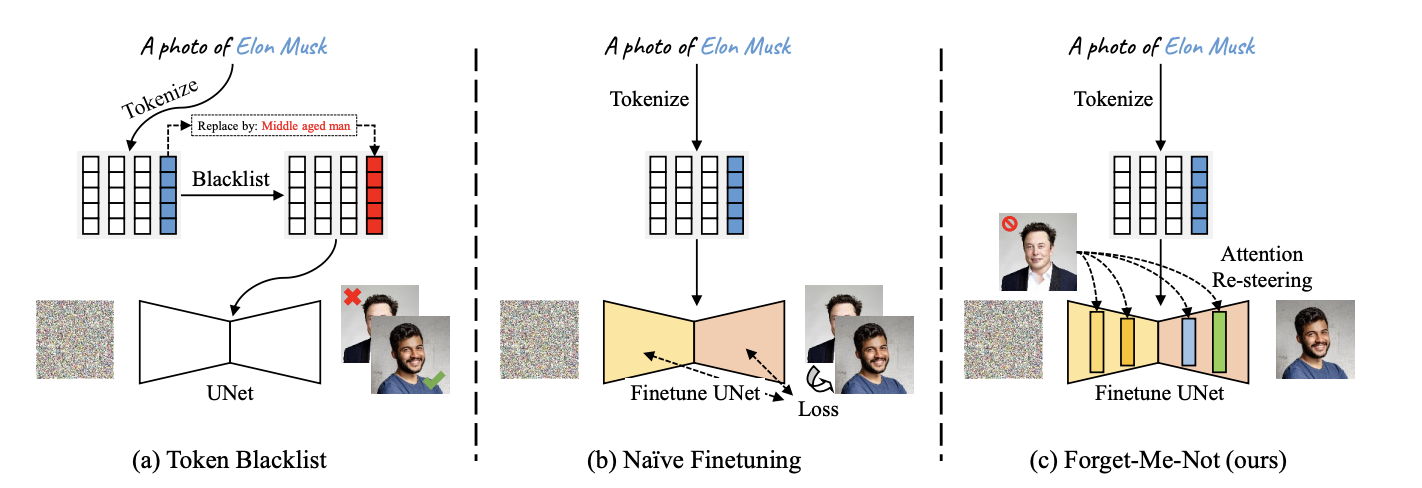
\includegraphics[width=1\textwidth]{images/concept_removal_comp.png}
    \caption{ This figure shows two baseline forgetting methods and our proposed Forget-Me-Not. The target concept to forget is Elon Musk.
    One baseline is (a) Token Blacklist that simply replaces the target token with a different one. The other baseline is (b) Naive Fintuning in
    which instead of replacing tokens, it finetunes model weights so that the new weights generate outputs containing unrelated concepts. Our
    method (c) Forget-Me-Not utilizes Attention Re-steering in which we finetune only UNet to minimize each of the intermediate attention
    maps associated with the target concepts to forget. \cite*{zhang2023forgetmenot}}
\end{figure}

